\documentclass[class=report, crop=false, 12pt,a4paper]{standalone}
\usepackage{enumitem}
\usepackage{multicol}
\usepackage{graphicx}
\usepackage{float}
\usepackage{amsmath}
\usepackage{amssymb}
\usepackage{mathtools}
\usepackage{siunitx}
\usepackage{commath}
\usepackage{array}
\usepackage{natbib}
\usepackage[a4paper,width=150mm,top=25mm,bottom=25mm]{geometry}
\setlength{\parindent}{0pt}
\setlength{\parskip}{1em}
\raggedbottom
\begin{document}
\chapter{Developing Impedance Diagram}
\section{Three Phase Power}
\subsection{Three-phase alternating voltages}
A three-phase synchronous generator consists of a rotor and a stator.
\begin{itemize}
	\item Adjusting excitation current on the rotating field will change the magnitude of the three AC phase emfs generated in the stator.
	\item Changing the rotational speed changes the frequency of the AC emfs
	\item The three phases generated are \SI{120}{\degree} displaced due to special arrangement
\end{itemize}
\subsection{Three-phase emfs (or terminal voltages) can be expressed mathematically}
\begin{align}
	v_a\left( t\right) & = V_m \sin\left( \omega t\right)                  \\
	v_b\left( t\right) & = V_m \sin\left( \omega t - \frac{2\pi}{3}\right) \\
	v_c\left( t\right) & = V_m \sin\left( \omega t - \frac{4\pi}{3}\right)
\end{align}
$V_m$ is the peak (maximum) voltage, $\omega$ is the angular frequency, $t$ is time. The phase displacement between the three-phase waveforms is \SI{120}{\degree} or $\frac{2\pi}{3}$ radians. $v_a$, $v_b$ and $v_c$ are the three phase voltages.
\subsection{Three-phase, six-wire connection}
The are different arrangements for distributing three-phase electrical power. The three phases can be independent of each other as seen below and treated as three separate circuits. This is known as the \textit{three-phase, six-wire system}.
\begin{figure}[H]
	\centering
	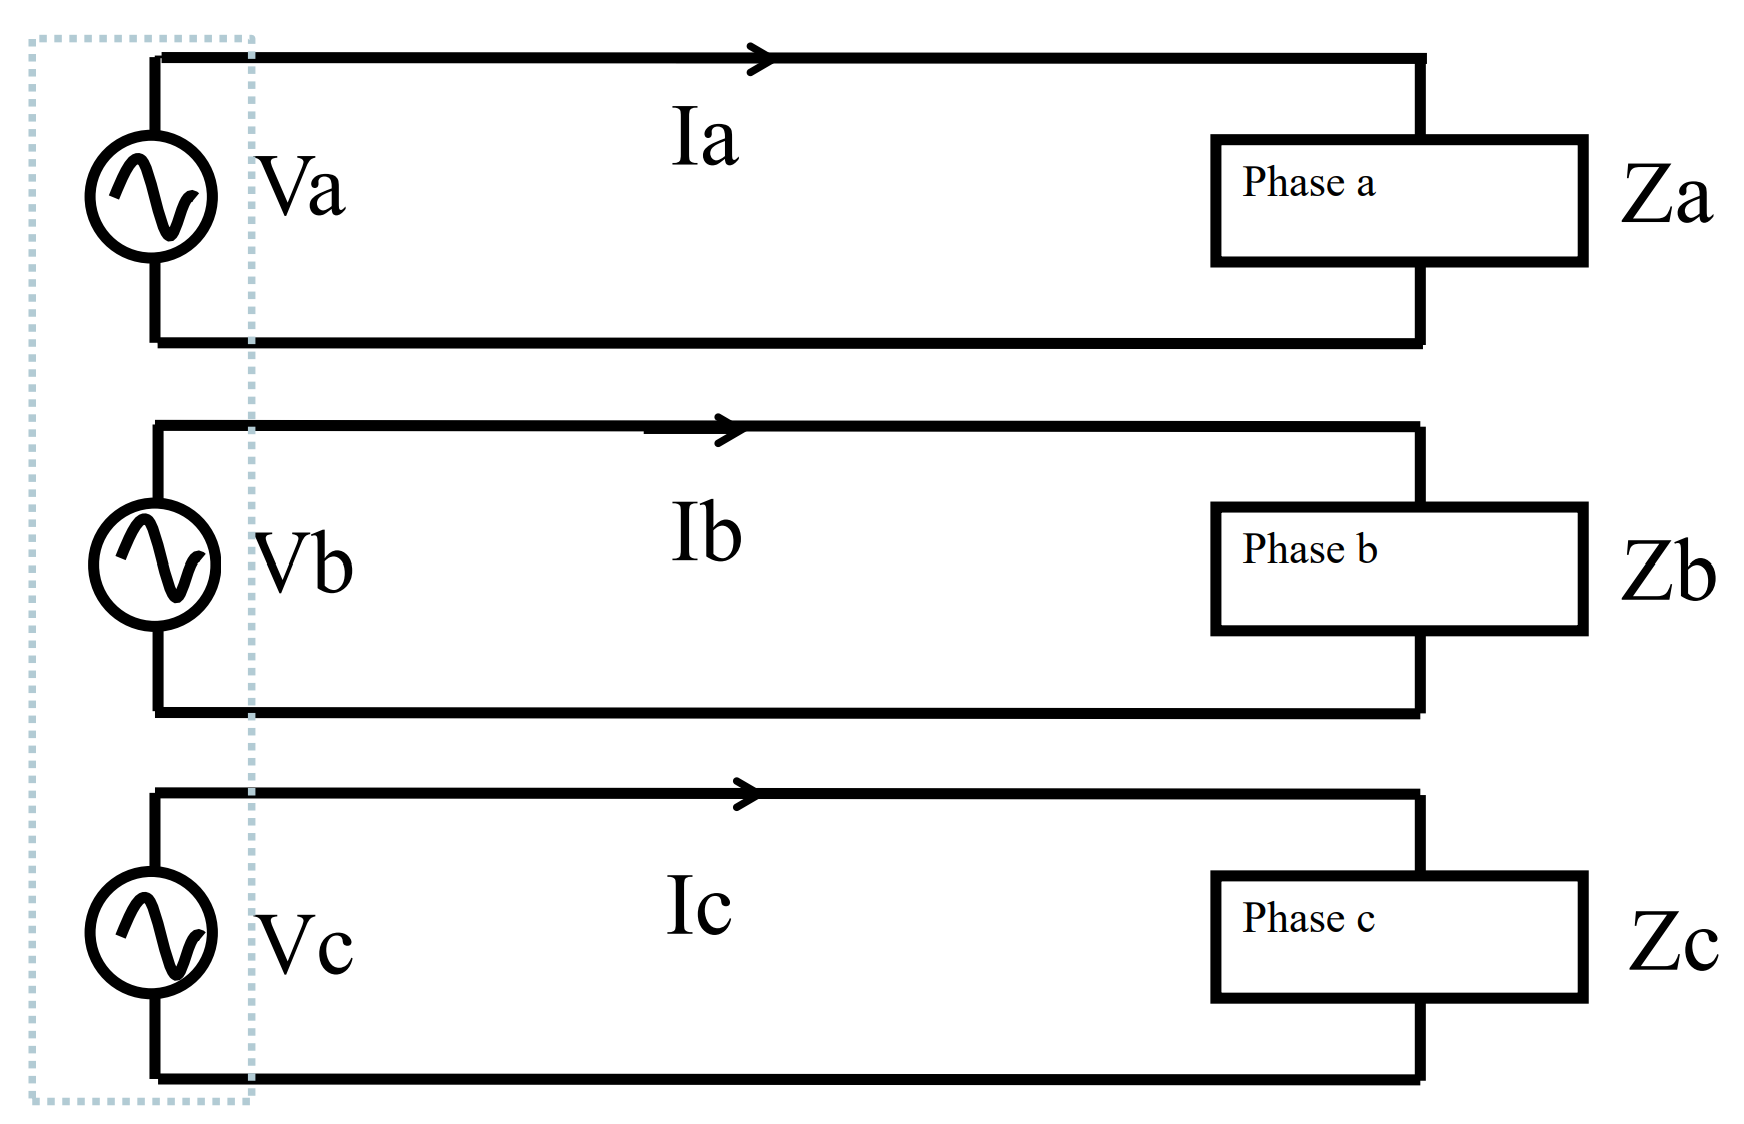
\includegraphics[width = 0.9\textwidth]{../img/figure6.png}
	\caption{Three-phase, six-wire system.}
\end{figure}
\subsection{Three-phase current}
\begin{quote}
	The currents flow in a three-phase circuit when there is a three-phase load. We will initially assume that the three-phase load is balanced i.e. the magnitude of voltage, current and the phase-angle is the same for each phase circuit. This is not true for three-phase circuits with unbalanced loads and the mathematical approach is different and more complex so we will examine this later.
\end{quote}
\subsection{Three-phase alternating current}
The currents associated with a three-phase system that flow from the supply to the load may be described mathematically by:
\begin{align}
	i_a \left(t\right) & = I_m \sin \left( \omega t + \theta \right)                \\
	i_b \left(t\right) & = I_m \sin \left( \omega t - \frac{2\pi}{3} +\theta\right) \\
	i_c \left(t\right) & = I_m \sin \left( \omega t - \frac{4\pi}{3} +\theta\right)
\end{align}
Note: the phase displacement angle ($\theta$) can be positive (leading PF) indicating a capacitive load or negative (lagging PF) indicating an inductive load. A zero phase displacement angle indicates a resistive circuit or a circuit at resonance ($X_L = X_C$).
\subsection{Connecting Three-Phases}
A three-phase six wire system is generally expensive to install and is actually unnecessary due to an inherent balancing characteristic.

In the balanced three-phase system, the algebraic sum of voltage at any point where all three-phase voltages are connected is zero.

The zero voltage point is known as the `star point' and this may be grounded or left isolated (floating). In most electrical systems the star point is grounded with exceptions being some ship types.
\subsection{Star and delta connections}
The number of transmission wires can be reduced by connecting the phases in either delta or star configuration.
\begin{figure}[H]
	\centering
	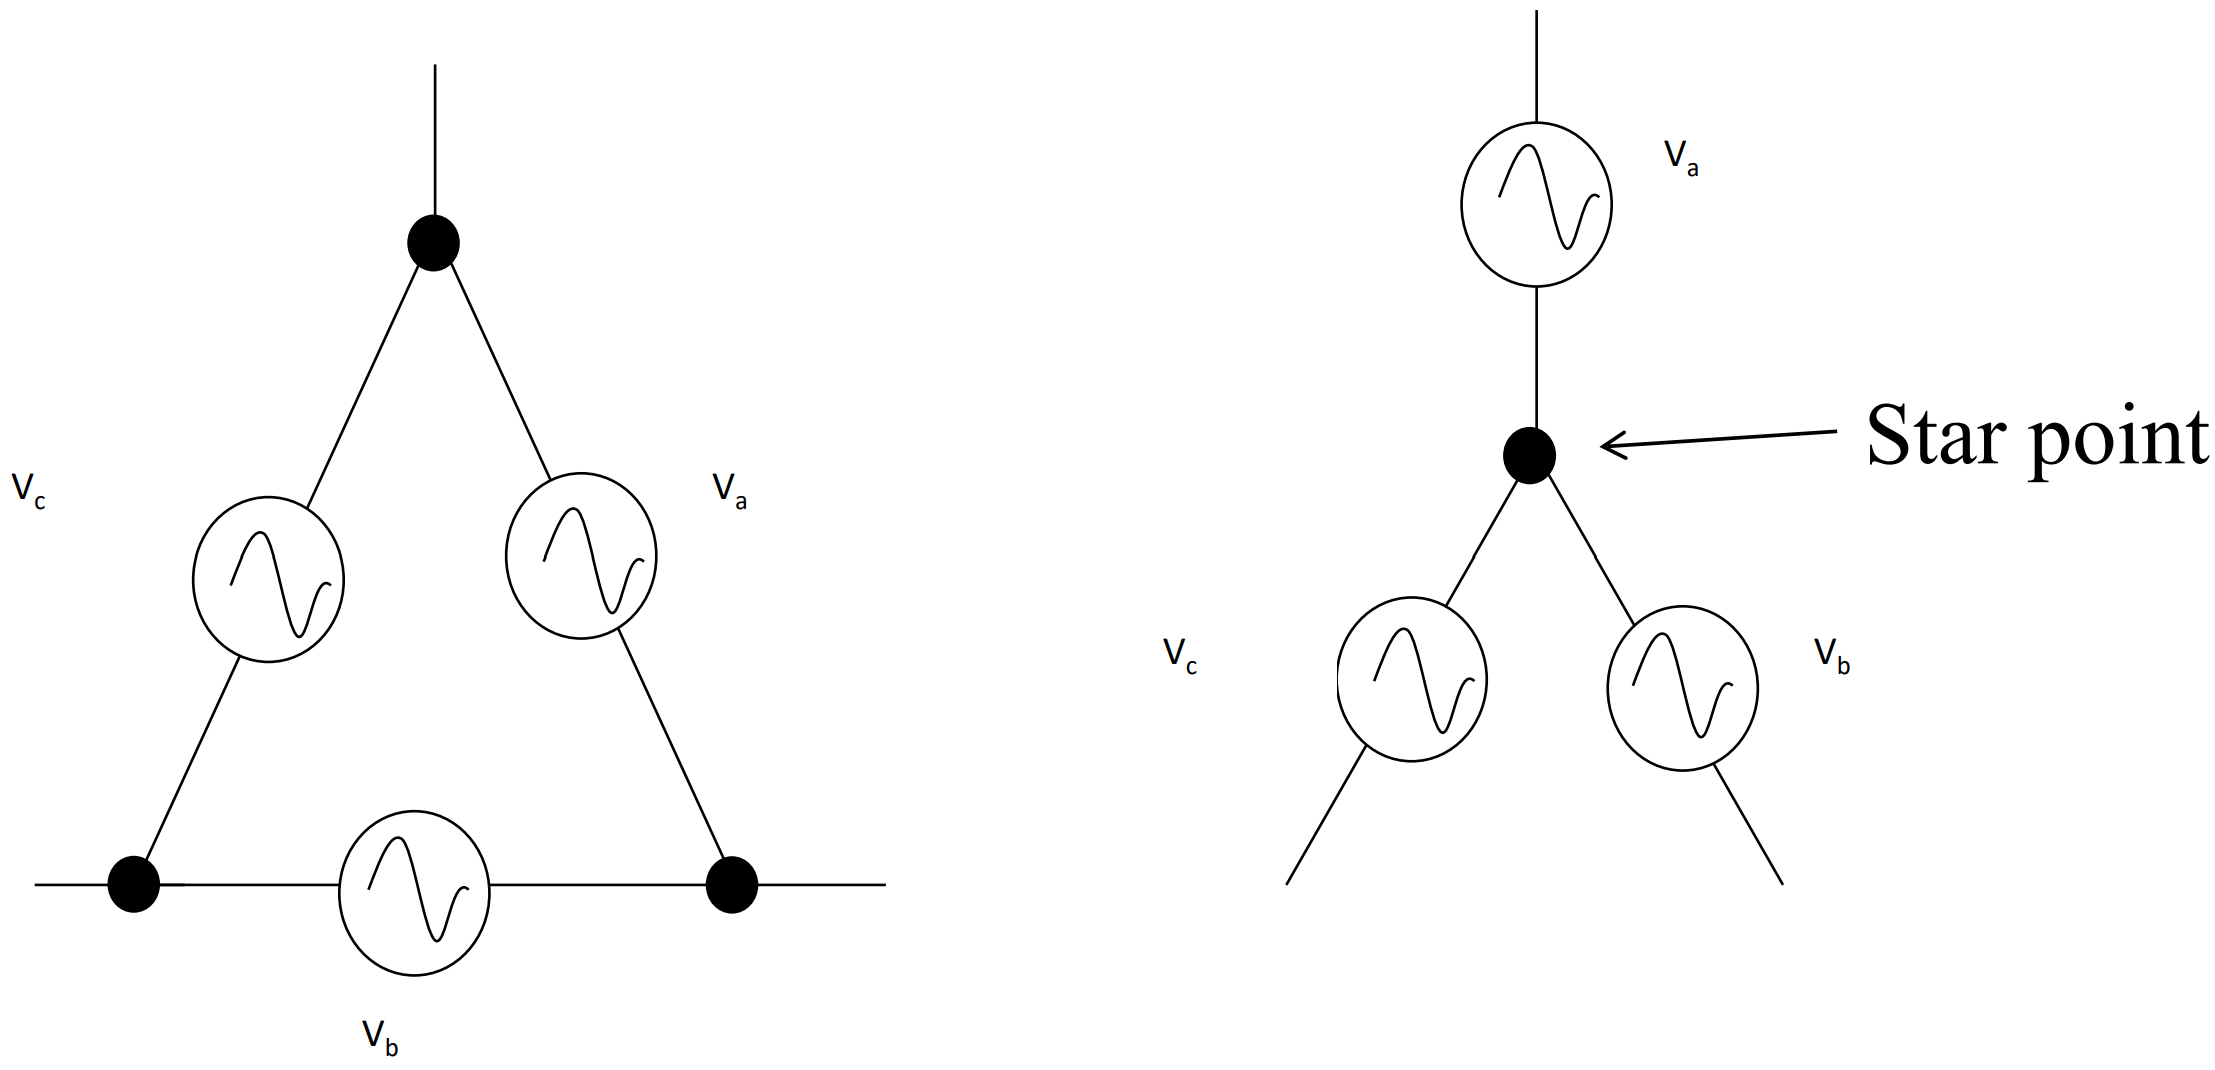
\includegraphics[width = \textwidth]{../img/figure7.png}
	\caption{Star and delta configurations.}
\end{figure}
\begin{figure}[H]
	\centering
	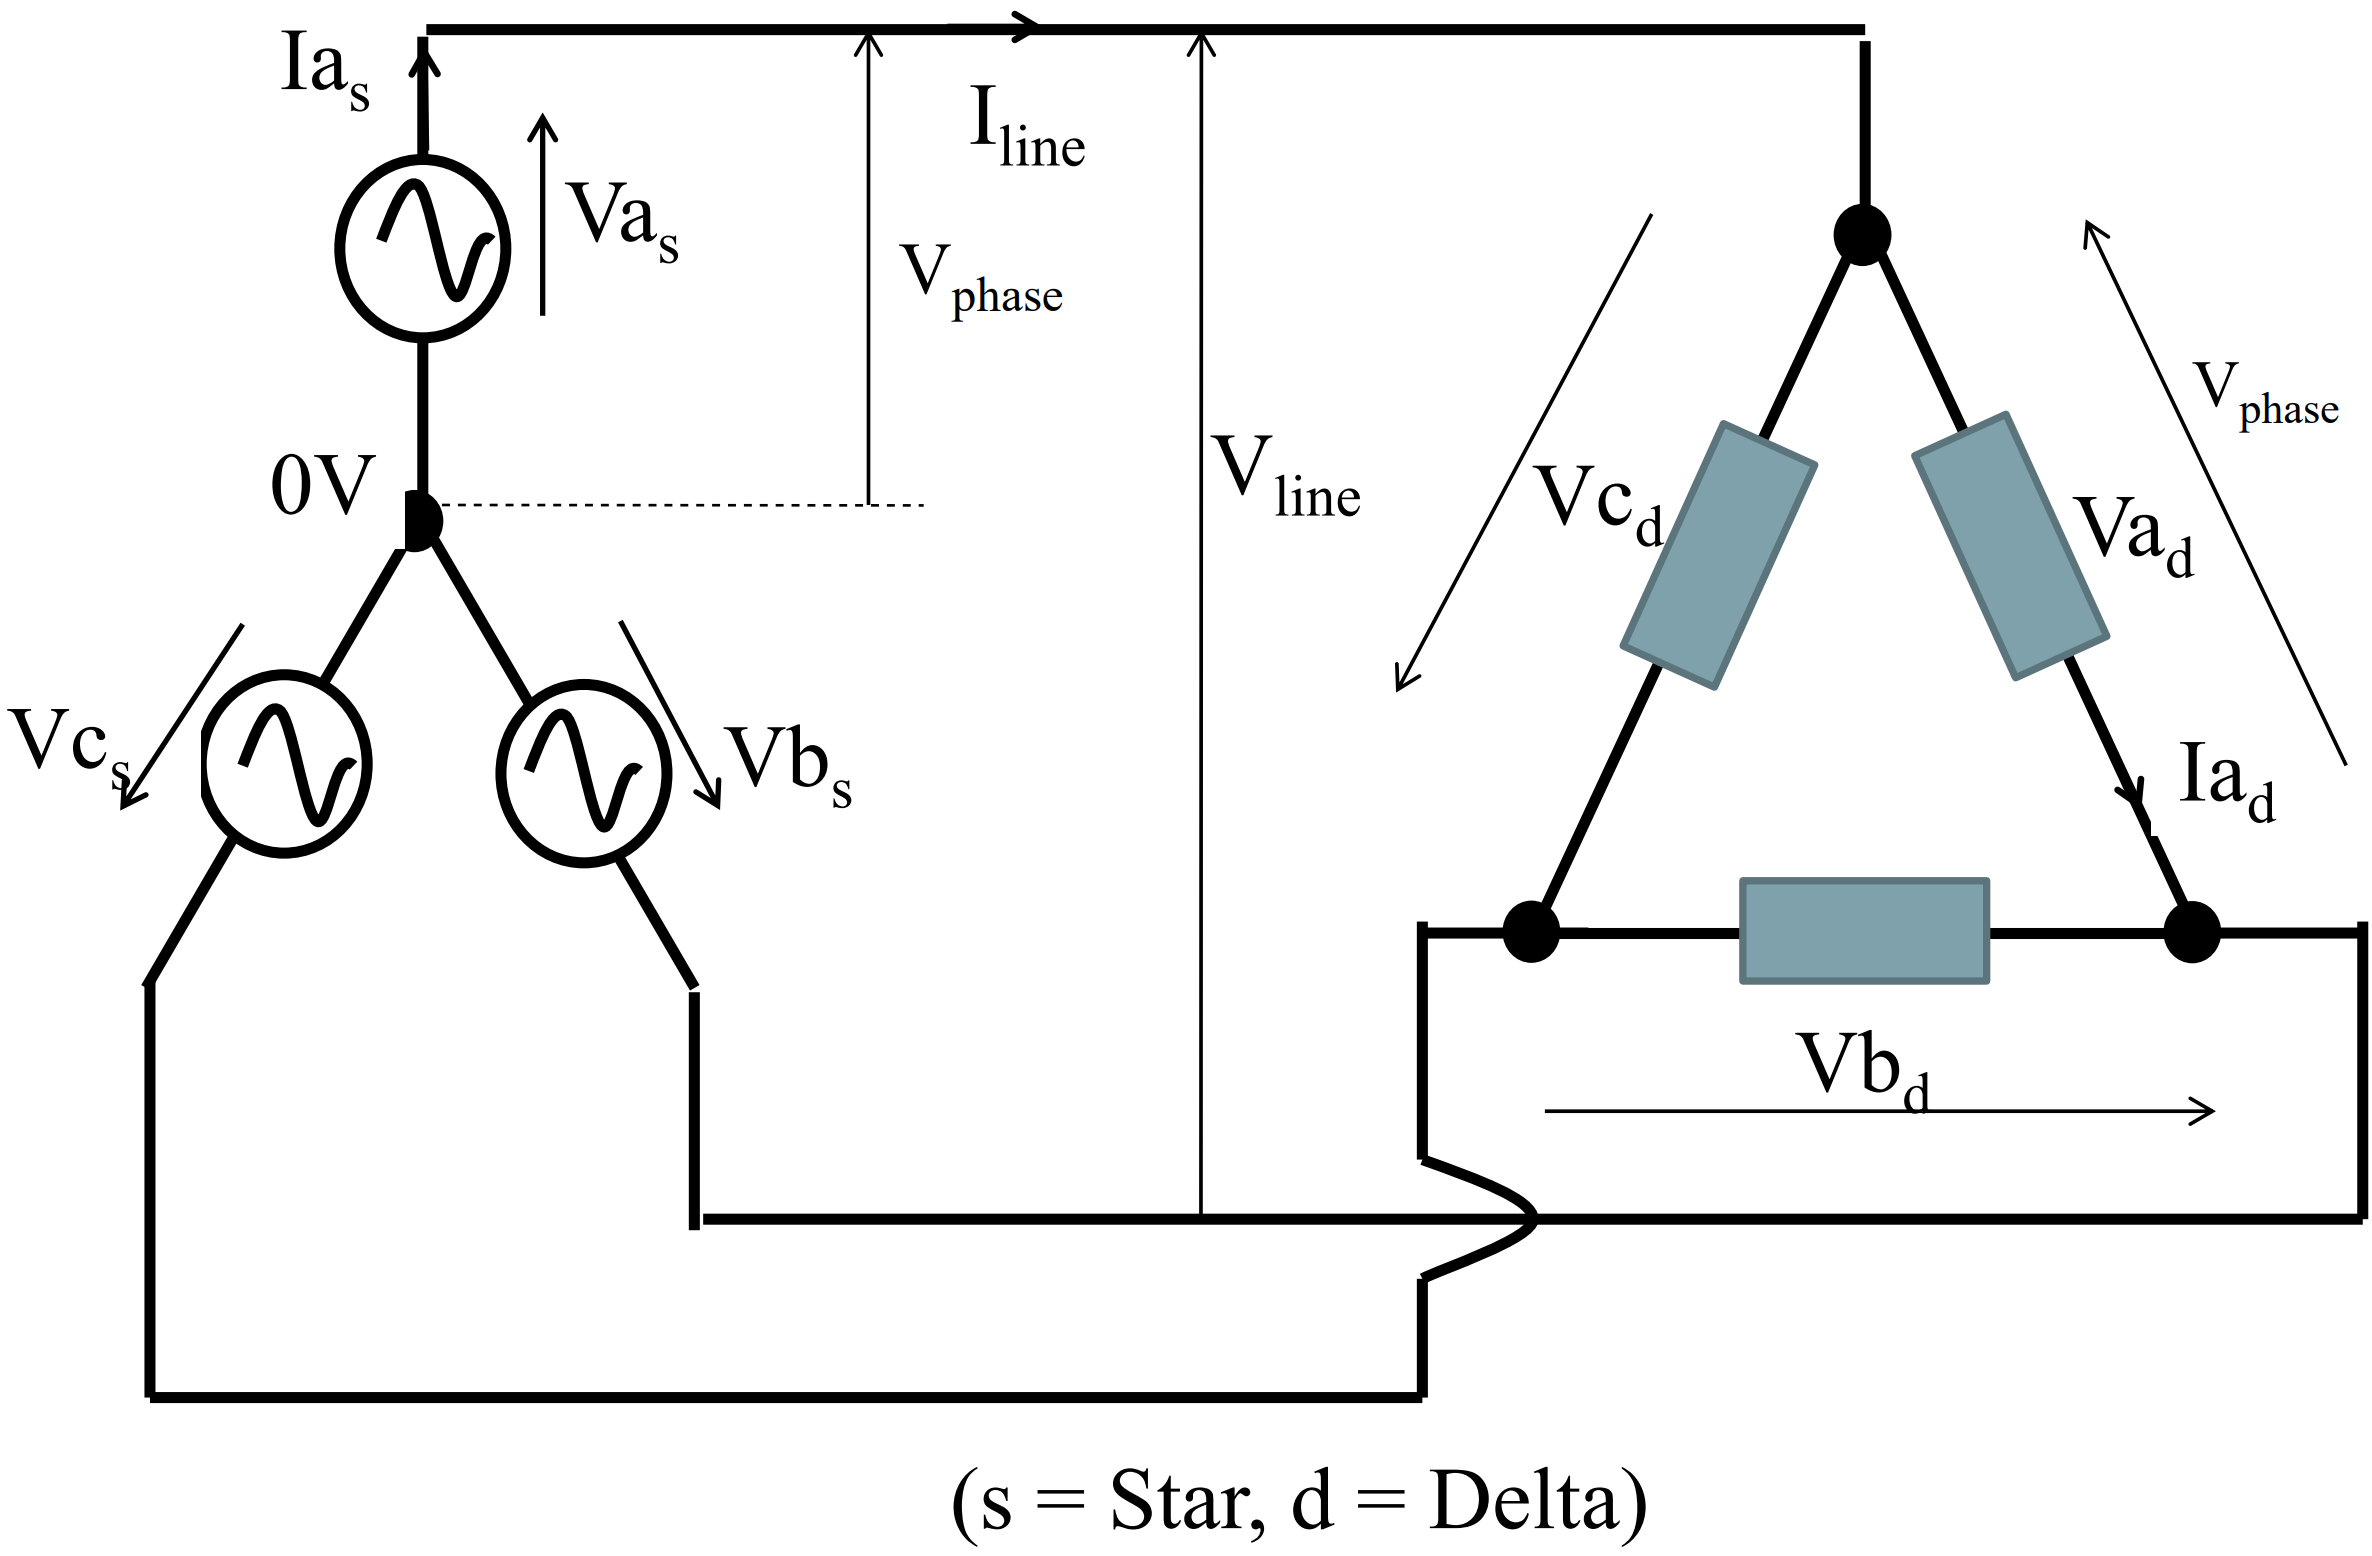
\includegraphics[width = \textwidth]{../img/figure8.png}
	\caption{Star generator and delta load.}
\end{figure}
\subsection{Phase and line voltages}
There are therefore two voltage types (either generated as a potential difference) when considering three-phase circuits. These are commonly known as the \textit{phase voltage} and \textit{line voltage}.

The phase voltages in the star-delta circuit are as follows:
\begin{itemize}
	\item $Vas$, $Vbs$, $Vcs$ for the star circuit
	\item $Vad$, $Vbd$, $Vcd$ for the delta circuit
\end{itemize}
The line voltages can be measured as follows:
\begin{align}
	Vab & = Vas - Vbs = Vad \\
	Vbc & = Vbs - Vcs = Vbd \\
	Vca & = Vcs - Vas = Vcd
\end{align}
and if the line voltages measure is reversed:
\begin{align}
	Vba & = Vbs - Vas = -Vad \\
	Vcb & = Vcs - Vbs = -Vbd \\
	Vac & = Vas - Vcs = -Vcd
\end{align}
Which is why a three-phase system is known as a six-pulse system - (important in power electronic systems).
\subsection{Relationships between star and delta}
For the delta arrangement:
\begin{align}
	V_p & = V_l                  \\
	I_p & = \frac{I_l}{\sqrt{3}}
\end{align}
For the star arrangement:
\begin{align}
	V_p & = \frac{V_l}{\sqrt{3}} \\
	I_p & = I_l
\end{align}
Where $I_p$ and $V_p$ are the phase currents and voltages and $I_l$ and $V_l$ are the line currents and voltages respectively. Note: Delta is also known as `mesh'; Star is also known as `Y'.
\subsection{Single-phase impedance triangle}
\begin{figure}[H]
	\centering
	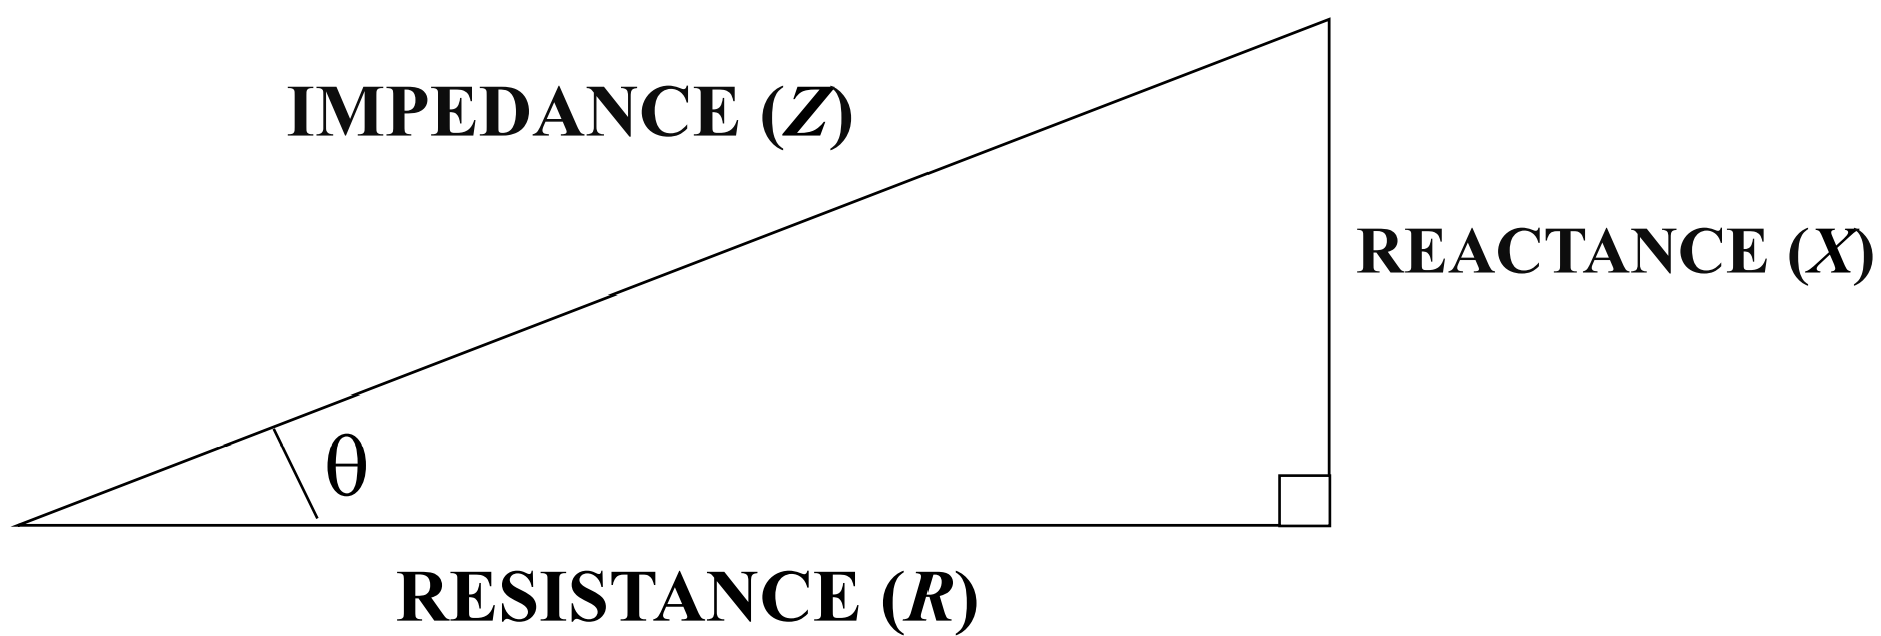
\includegraphics[width = 0.8\textwidth]{../img/figure9.png}
	\caption{Single-phase impedance triangle.}
\end{figure}
\begin{align}
	Z & = R + jX                                          \\
	  & = R + j\left(X_L - X_C\right)                     \\
	  & = R + j\left(\omega L - \frac{1}{\omega C}\right)
\end{align}
Where, $Z$ is impedance, $R$ is resistance, $X_L$ is inductive reactance, $X_C$ is capacitive reactance, $\omega$ is angular frequency ($2\pi f$).
\subsection{Single-phase power triangle}
\begin{figure}[H]
	\centering
	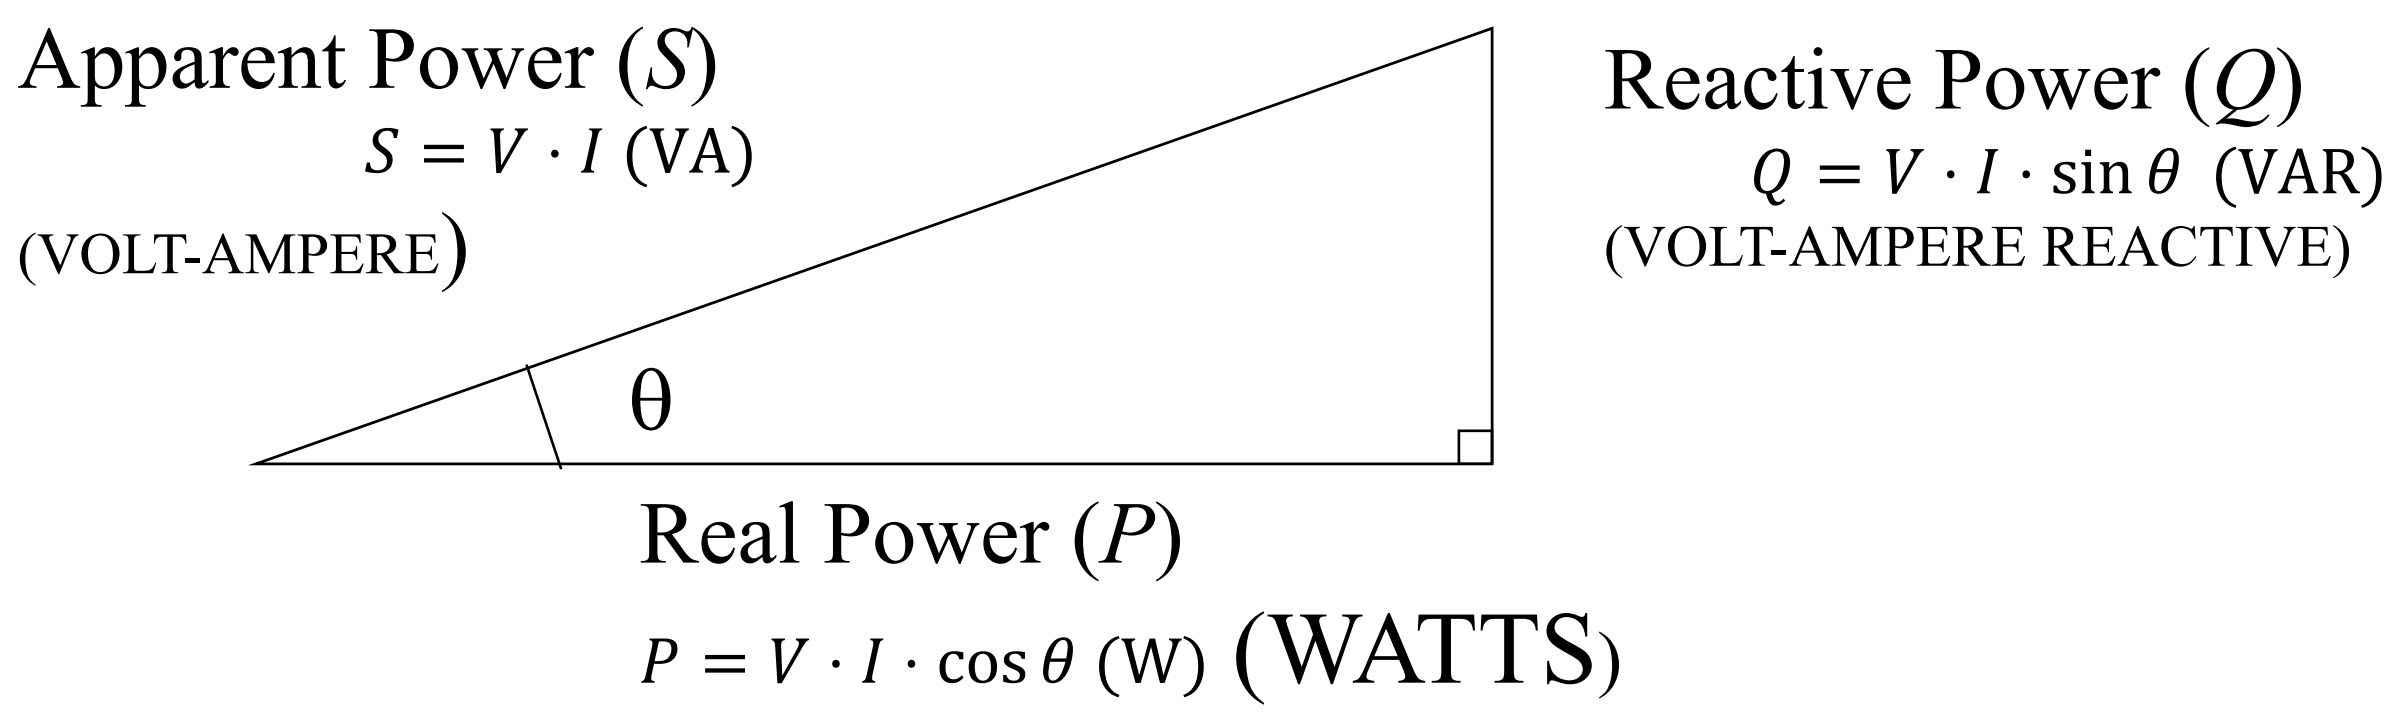
\includegraphics[width = 0.8\textwidth]{../img/figure10.png}
	\caption{Single-phase power triangle.}
\end{figure}
\begin{itemize}
	\item Real power ($P$) is the power that can be put into or taken from the electrical system and is measured in Watts (\si{\watt}).
	\item Reactive power ($Q$) is the power that circulates in the electrical system and is measured in Volt-Ampere-Reactive (VAR).
	\item Apparent power ($S$) is what is apparent from the product of voltage and current and is measured in Volt-Amperes (VA).
\end{itemize}
\subsection{Three-phase power}
Since $V$ in the star circuit and $I$ in the delta circuit is subject to change simply by dividing by $\sqrt{3}$, whilst the other variable $I$ and $V$ in star and delta respectively remain unchanged. Hence we get:
\begin{gather}
	P = \sqrt{3} \cdot I_{line} \cdot V_{line} \cdot \cos \theta
\end{gather}
For apparent power ($S$) and reactive power ($Q$) we have:
\begin{align}
	S & = \sqrt{3} \cdot I_{line} \cdot V_{line}                   \\
	Q & = \sqrt{3} \cdot I_{line} \cdot V_{line} \cdot \sin \theta
\end{align}
\subsection{Student Activity}
Three coils each of resistance \SI{5}{\ohm} and inductive reactance of \SI{10}{\ohm} are connected in (a) star and (b) delta across a \SI{440}{VRMS} three-phase (line) supply.

If each coil has a capacitor connected in parallel having capacitive reactance of \SI{20}{\ohm} then calculate the line and phase currents and the total power absorbed.
\section{Per Unit (PU) System}
\subsection{Electrical line diagram to Impedance diagram}
\begin{itemize}
	\item The \textit{`electrical line diagram'} - a schematic which allows an understanding of equipment and system arrangements.
	\item The \textit{`impedance diagram'} - a schematic which allows an understanding of the equipment and system impedances.
	\item The layout of both the `electrical line diagram' and `impedance diagram' should be similar but in the `impedance diagram' all equipment and lines are replaced with impedances.
	\item All impedances will need to be calculated to a \textit{common base} - hence use of a per unit system.
\end{itemize}
\subsection{Simple equivalent impedances}
For the purposes of steady-state analysis the Electrical Line Diagram is converted to an `Impedance Line Diagram' where the equipment is represented as an `Equivalent Impedance'. Typical \textit{simple} impedances representing equipment are: (note: not all $R$, $L$ and $C$ values may be given).
\begin{figure}[H]
	\centering
	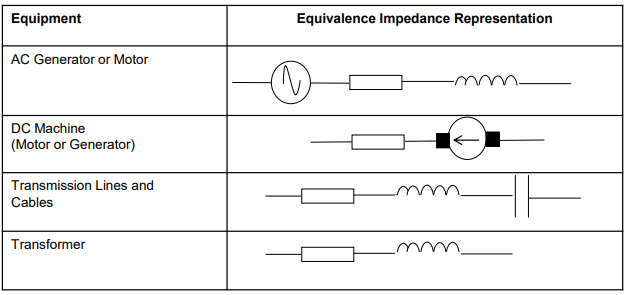
\includegraphics[width = \textwidth]{../img/figure11.png}
	\caption{Equivalent Impedance Representations.}
\end{figure}
\subsection{How manufacturers of electrical equipment specify ratings}
Manufacturers of electrical equipment would usually specify electrical equipment as follows:

e.g. A synchronous generator
\begin{itemize}
	\item S = 10 MVA (value of apparent power)
	\item V = 3.3 kV (line voltage rating of the equipment)
	\item Phase = 3 (number of phases)
	\item PF = 0.8 (usual value of power factor of equipment)
	\item N = 1500 rpm (design speed of rotation)
	\item F = 50 Hz (frequency of the alternating current \& voltage)
	\item X = 0.14 (Reactance given as a pu value or as a \%)
	\item Connection = star (stator windings)
\end{itemize}
\subsection{The per unit system}
In Electrical Power System Analysis the per unit system is the preferred method for analysing circuit behaviour rather than the standard SI system of units (Watts, Volts, Amperes, etc.)

The advantages of the per unit system are:
\begin{itemize}
	\item Computations for power systems have several voltage levels because of connected transformers is very cumbersome when using the SI system because values need to be referred across the transformer turns ratio. The per unit system (overcomes or simplifies) this problem.
	\item All powers, voltage, currents and impedances are expressed as per unit values of specified base values. This means they are easily compared with one another which is very helpful for equipment specification and selection and in power system design and its analysis.
\end{itemize}
\subsection{Values in per unit system}
In the per unit system five base values are needed. These are \textbf{power, current, voltage, impedance} and \textbf{power factor}. It is necessary to choose two base values and to calculate two base values.

Usually the base values defined are:
\begin{itemize}
	\item the Apparent Power (Base VA)
	\item Voltage (Base V)
\end{itemize}
Power Factor is already expressed in per unit form. Once the base values are calculated then `actual values' in the circuit can be expressed in per unit form.
\end{document}













